%%%%%%%%%%%% Preamble %%%%%%%%%%%%
\documentclass[11pt,letterpaper,oneside]{article} %Change basic font size and paper size here.
\usepackage{setspace, graphicx, fullpage, fancyhdr, amssymb, amsmath, epsfig, natbib, array, multirow, hyperref, tabularx, lscape, booktabs, sidecap, subfig, longtable, enumitem}
% Not all packages are actually used to compile this document. 
% This is just the set of packages that I work with most often.
% If MikTeX asks you to install them, just agree.

\usepackage[
top    = 2cm,
bottom = 2cm,
left   = 2cm,
right  = 2cm]{geometry}

\usepackage[font=small]{caption} % Font size for captions

\hypersetup{
    bookmarks=false,         % show bookmarks bar?
    unicode=false,          % non-Latin characters in Acrobat?s bookmarks
    pdftoolbar=true,        % show Acrobat?s toolbar?
    pdfmenubar=true,        % show Acrobat?s menu?
    pdffitwindow=false,     % window fit to page when opened
    pdfstartview={FitH},    % fits the width of the page to the window
    pdftitle={},    % title
    pdfauthor={},     % author
    pdfsubject={Subject},   % subject of the document
    pdfcreator={Creator},   % creator of the document
    pdfproducer={Producer}, % producer of the document
    pdfkeywords={keywords}, % list of keywords
    pdfnewwindow=true,      % links in new window
    colorlinks=true,       % false: boxed links; true: colored links
    linkcolor=blue,          % color of internal links
    linkbordercolor={0 0 0},  %border color
    citebordercolor={0 0 0},
    citecolor=blue,        % color of links to bibliography
    filecolor=black,      % color of file links
    urlcolor=blue,         % color of external links
}

%%%%%%%%%%%% Main Body %%%%%%%%%%%%
\begin{document}

%%%% Title %%%%
\pagestyle{plain} %Basic options are plain (just page num) empty (no page num, no headers) and fancy.
\title{\small\textsc{POIR {\LaTeX} Workshop} \\
	\Large{Basic \texttt{article} style template}}
\author{Therese Anders (\href{mailto:tanders@usc.edu}{tanders@usc.edu})} 
\date{\today}
\maketitle % This creates the title at the top of the document.

\singlespacing

\tableofcontents %Note that all indexing and cross-referencing is only done upon the second compiling.

\newpage % Equivalent to Word's page break.
\section{Text and formatting}
\doublespacing
\textit{Lorem ipsum dolor sit amet}, \textbf{consectetur adipiscing elit}. \underline{Praesent volutpat dictum commodo}. \textsc{Mauris dignissim sagittis orci eu viverra}. Maecenas sollicitudin libero vel augue blandit hendrerit. \texttt{Praesent id blandit orci}. Proin velit mauris, fermentum vitae ornare ut, vulputate et augue. Mauris a eros et velit tempus commodo. In hac habitasse platea dictumst. Suspendisse sodales purus nec nisl dapibus tristique. Suspendisse potenti.

\singlespacing
Morbi at scelerisque orci, ac sagittis justo. Aenean cursus mi maximus purus condimentum, at dictum tellus cursus. Nulla et lectus a risus dictum feugiat nec vitae odio. Proin arcu ex, sodales vel malesuada nec, lobortis ut orci. Morbi vel libero orci. Donec vehicula vitae libero sed pellentesque. Vivamus posuere dapibus dolor vitae semper. Curabitur imperdiet a massa nec mollis. Praesent rhoncus magna eget consequat laoreet. Donec congue cursus augue non scelerisque. {\tiny Integer et mi sit amet odio consectetur}                dapibus. %Note the function of white space.

\begin{Large} %See what happens if you use lower case here.
\begin{center}
General advise: Have an easy hand with these formatting options. {\LaTeX} is pretty good at selecting size patterns and spacing that is aesthetically pleasing. Especially in the beginning, limit yourself to choosing your paper size, basic font size, and spacing, and let {\LaTeX} do the rest.
\end{center}
\end{Large}

\normalsize

\section{Lists}
\subsection{Bullet Points}
\begin{itemize}
\item Point 1.
\item Bla bla.
\item More bla bla.
\end{itemize}

\subsection{Numbered lists}
\begin{enumerate}
\item This is the most important.
\item Less important.
\item Even less.
\end{enumerate}

\subsection{Nested lists}
\begin{itemize}
\item Some stuff.
	\begin{enumerate}
	\item Oh first point.
	\item Second point.
	\end{enumerate}
\item Back to stuff.
\end{itemize}

\section{Math Symbols}
{\LaTeX} has beautiful math typesetting capabilities.\footnote{For a list of the most common math symbols, see \url{http://web.ift.uib.no/Teori/KURS/WRK/TeX/symALL.html}.} We can either write functions and math symbols in text using the \$ sign as a wrapper. So for example, if you love Greek letters, you can just write them in text like this $w_{i,t} = \alpha v_{i, t-1} + \beta x_{i, t-1} + \delta_t + \gamma_i + \epsilon_{i, t}$. For longer functions, use the following wrapper:
\begin{equation}
\frac{\partial EU_{ns_p}}{\partial v}=A'(v)-A'(v)(g+v-s-n_L)f\gamma-A(v)f\gamma-B'(v)\leq0\gamma-B''(v)
\end{equation}
\begin{equation}
\frac{\partial^2 EU_{ns_p}}{\partial v^2}=A''(v)-A''(v)(g+v-s-n_L)f\gamma-A'(v)f\gamma-A'(v)f\gamma-B''(v)
\end{equation}

\section{Figures}
{\LaTeX} puts figures and tables into so-called \textbf{floats}. Floats are containers for content that cannot be broken over a page. The algorithm determines the optimal placement of the float on the page and the text around it. This is a blessing and a curse. Floats are one of the reason that make {\LaTeX} documents pretty. But trying to force {\LaTeX} to place a figure in a position it does not deem optimal can be a hassle. Notice how Figure \ref{graph1} changes position as we add and remove content from our document.

\begin{figure}[!h] 
\begin{center}
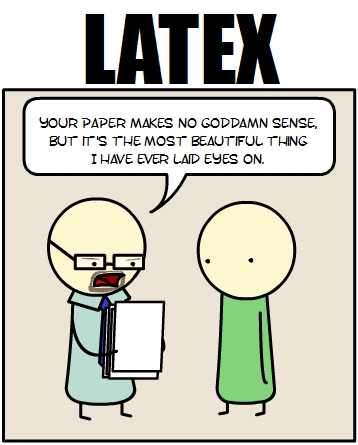
\includegraphics[width = 2in]{latex_comic.jpg}
\caption{Source \url{http://bit.ly/25VwZaG}.}
\label{graph1}
\end{center}
\end{figure}


There are some ways to ``friendly force'' %Note here how quotation marks are created!
% Also note how LaTeX ignores single returns.
{\LaTeX} to comply with your wishes, such as the commands \texttt{h} (here),  \texttt{t} (top),  \texttt{b} (bottom), and  \texttt{p} (page), as well as the infamous  \texttt{!} (no, really!). {\LaTeX} may or may not comply with your wishes. There are ways to truly force specific positions on the program, but we will not cover this here. 


\section{Tables}
Programming tables in {\LaTeX} from scratch is not straightforward. Examine the code below to understand the basic logic. The \texttt{tabular} is wrapped into a \texttt{table} float. Then follows a formatting operator, which tells the program to center the tabular on within the float. Upon initializing the tabular, we tell {\LaTeX} how many columns there are (3), that they should be right (r), center (c), and center (c) oriented, and that we want vertical lines ($|$). We then include the body of each row, with the \texttt{\&} symbol delimiting the content for each cell. Below, see the code that is used to create Table \ref{tab_prison}.
%Notice the use of the cross-referencing here. 
%I use \ref{} and the label of the table to place the link.

\begin{verbatim}
\begin{table}[!htbp]
  \centering
  \caption{The classic ``Prisoner's Dilemma"}
    \begin{tabular}{|r|c|c|}
    \hline
    {\bf Player I / Player II} & Cooperate & Defect \\
    \hline
    Cooperate & (5,5) & (-10, 10) \\
    \hline
    Defect & (10,-10) & (-5,-5) \\
    \hline
    \end{tabular}
  \label{tab_prison}
\end{table}
\end{verbatim}

\begin{table}[!htbp]
  \centering
  \caption{The classic ``Prisoner's Dilemma"}
    \begin{tabular}{|r|c|c|}
    \hline
    {\bf Player I / Player II} & Cooperate & Defect \\
    \hline
    Cooperate & (5,5) & (-10, 10) \\
    \hline
    Defect & (10,-10) & (-5,-5) \\
    \hline
    \end{tabular}
  \label{tab_prison}
\end{table}

Fortunately, there are a number of tools that make it much easier to create tables in {\LaTeX}. For example, Table \ref{tabfancy} was created using the \texttt{stargazer} package in \texttt{R} and imported into the {\LaTeX} document using the \texttt{input} command. A similar output can be achieved using the \texttt{estaout} in Stata.

% Table created by stargazer v.5.2 by Marek Hlavac, Harvard University. E-mail: hlavac at fas.harvard.edu
% Date and time: Tue, Feb 06, 2018 - 11:49:42
\begin{table}[!htbp] \centering 
  \caption{Table created with R's stargazer package.} 
  \label{} 
\scriptsize 
\begin{tabular}{@{\extracolsep{0pt}}lcc} 
\\[-1.8ex]\hline 
\hline \\[-1.8ex] 
 & \multicolumn{2}{c}{\textit{Dependent variable:}} \\ 
\cline{2-3} 
\\[-1.8ex] & Internet Users & Life Expectancy \\ 
\\[-1.8ex] & (1) & (2)\\ 
\hline \\[-1.8ex] 
 Polity Score & 0.0842$^{***}$ &  \\ 
  & (0.0202) &  \\ 
  Population & 0.0000 &  \\ 
  & (0.0000) &  \\ 
  GDP p.c. & 0.0010$^{***}$ & 0.0005$^{***}$ \\ 
  & (0.00002) & (0.00001) \\ 
  Constant & 5.9550$^{***}$ & 62.5757$^{***}$ \\ 
  & (0.4082) & (0.1602) \\ 
 \hline \\[-1.8ex] 
Observations & 3,003 & 4,111 \\ 
R$^{2}$ & 0.3839 & 0.3343 \\ 
Adjusted R$^{2}$ & 0.3833 & 0.3341 \\ 
Residual Std. Error & 17.9527 (df = 2999) & 8.6253 (df = 4109) \\ 
\hline 
\hline \\[-1.8ex] 
\textit{Note:}  & \multicolumn{2}{r}{$^{*}$p$<$0.1; $^{**}$p$<$0.05; $^{***}$p$<$0.01} \\ 
\end{tabular} 
\end{table} 


To manually create tables, you can use online generators, for example \url{http://www.tablesgenerator.com}.

\begin{center}
[Paste code generated with tablesgenerator here].
\end{center}

\section{Bibliographic Data}
One of the greatest things about using {\LaTeX} is the integration of bibliographies. Including citations into your documents is easy. First, you specify the desired citation format. There is a large number of citation styles out there, including the most common styles used by academic journals. When you need to change the citation format for submission to a journal, just download the respective style file and adjust the \texttt{\\bibliographystyle} parameter. Second, you specify the \texttt{.bib} to draw the bibliography from using the \texttt{\\bibliography} command. I use BibDesk as a citation manager that automatically creates the \texttt{.bib} file, but there are many other options. 

\begin{footnotesize}
\begin{verbatim}
\bibliographystyle{chicago}
\bibliography{/Users/thereseanders/Documents/UNI/USC/Resources/Latex/LaTeXWorkshop/sample_bib.bib}
\end{verbatim}
\end{footnotesize}

In this example we use the \texttt{natabib} package for citation management. For more information, see \url{https://en.wikibooks.org/wiki/LaTeX/Bibliography_Management#Bibliography_styles}. Here is an overview over the most common \texttt{natbib} commands:

\begin{verbatim}
\citet{jon90} 	    -->    	Jones et al. (1990)
\citet[chap. 2]{jon90} 	    -->    	Jones et al. (1990, chap. 2)
\citep{jon90} 	    -->    	

(Jones et al., 1990)
\citep[chap. 2]{jon90} 	    -->    	(Jones et al., 1990, chap. 2)
\citep[see][]{jon90} 	    -->    	(see Jones et al., 1990)
\citep[see][chap. 2]{jon90} 	    -->    	(see Jones et al., 1990, chap. 2)
\citet*{jon90} 	    -->    	Jones, Baker, and Williams (1990)
\citep*{jon90} 	    -->    	(Jones, Baker, and Williams, 1990)
\end{verbatim}

Now, if you want to put the \citeauthor{waltz1979}s and the \citeauthor{vasquez1997}s of the world into conversation with each other, you can! But does any of this matter when, really, its all about institutions \citep{keohane2005}? As \citet{risse2000} says, ``Let's argue!'' 

\bibliographystyle{chicago}
\bibliography{sample_bib.bib}


% Double click on the .bib file in your folder to see what it looks like.

\end{document} %If this is missing, the document won't compile
%% EOF

%%% Additional Notes %%%
This shows that nothing will be printed after you place the \end{document} wrapper.

Look at the auxiliary files that LaTeX creates when compiling your document. 
You don't need to worry about specifics, just notice them and know that all you really need is your .tex file (for example when sharing a document).


